\section{Empirical results}

\subsection{Evaluating HPS under model and covariate shifts}

\begin{figure}[!t]
	\begin{subfigure}[b]{0.33\textwidth}
		\centering
		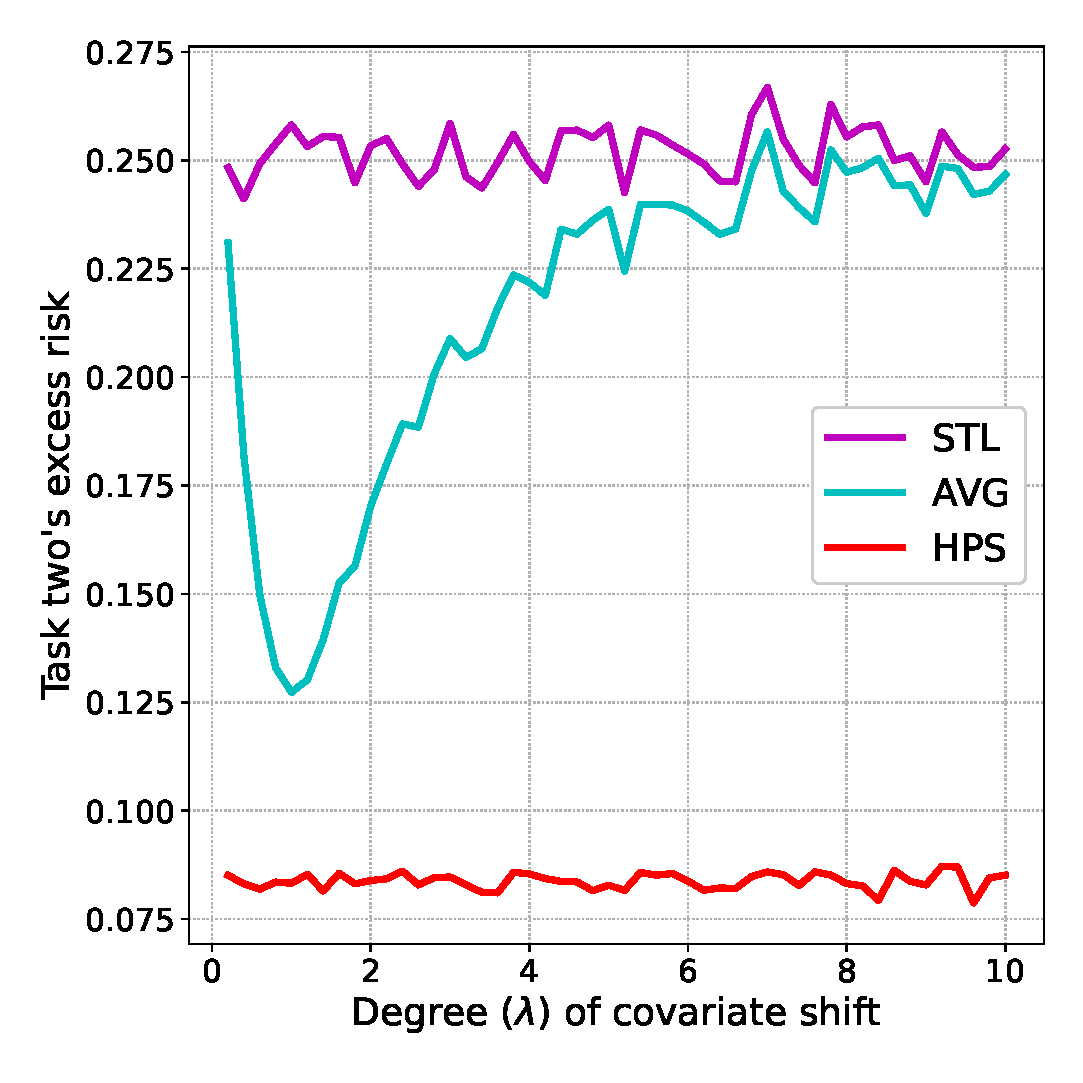
\includegraphics[width=0.98\textwidth]{figures/compare_risk_covariate_shift.eps}
		\caption{Covariate shift}
		\label{fig_sec5_covariate}
	\end{subfigure}
	\caption{Comparing HPS to several natural estimators for transfer learning. We find that HPS enjoys superior performance under covariate and/or model shifts. The results are averaged over five random seeds.}
	\label{fig_sec51}
\end{figure}

We show that HPS estimators enjoy superior empirical performance compared to several natural transfer learning estimators.
We consider the following estimators for this comparative study:
\begin{itemize}
    \item {\bf Averaging estimator (AVG):} given two tasks, take a convex combination of their OLS estimators $b \cdot \hat{\beta}^{\STL}_1 + (1 - b) \cdot \hat{\beta}^{\STL}_2$.
    \item {\bf STL estimator (STL):} simply use the OLS estimator of task two $\hat{\beta}^{\STL}_2$ without using task one's data.
    \item {\bf Transfer learning estimator (TL):} simply use the OLS estimator of task one $\hat{\beta}^{\STL}_1$ without using task two's data.
\end{itemize}

Figure \ref{fig_sec51} shows the result under covariate and/or model shifts.
Figure \ref{fig_sec5_covariate} considers the same example as Figure \ref{fig_sec31}.
%    \begin{align}
%    L(\hat{\beta}^{\AV}(\lambda) ) &= \left[ 1+ \OO(p^{-1/2+c})\right] \cdot \lambda^2 \left\| (\Sigma^{(2)})^{1/2}(\beta^{(1)}-\beta^{(2)})\right\|^2 \nonumber \\
%    &+  \left[ 1+ \OO(p^{-1/2+c})\right] \cdot \sigma^2   \lambda^2 \bigtr{\Sigma^{(2)} [(X^{(1)})^\top X^{(1)}]^{-1}  }\nonumber\\
%    & + \left[ 1+ \OO(p^{-1/2+c})\right] \cdot \sigma^2  (1-\lambda)^2 \bigtr{\Sigma^{(2)} [(X^{(2)})^\top X^{(2)}]^{-1}  }  . \label{L_AVE_simple}
%    \end{align}
%    and
%    \begin{align}
%    L(\hat{\beta}_2^{\STL} ) &= \left[ 1+ \OO(p^{-1/2+c})\right] \cdot \sigma^2  \bigtr{\Sigma^{(2)} [(X^{(2)})^\top X^{(2)}]^{-1}  }  . \label{L_STL_simple}
%    \end{align}
    %Moreover, there exists a constant $C_0>0$ such that with high probability,
    %\be\label{loss_large}
    %g(a) > g(0) \quad \text{for all $a$ such that }|a|\ge C_0.
    %\ee
    %with high probability for any small constant $\e>0$.
    
 %With Lemma \ref{fact_tr}, we obtain that w.h.p.,
%\begin{align}
%L(\hat{\beta}_2^{\STL} ) &= \left[ 1+ \OO(p^{-1/2+c})\right] \cdot \frac{p \sigma^2 }{n_2-p}   , \label{L_STL_simple01}
%\end{align}
%and
%\begin{align}
%L(\hat{\beta}^{\AV}(\lambda) ) &= \left[ 1+ \OO(p^{-1/2+c})\right] \cdot \lambda^2 \left\| (\Sigma^{(2)})^{1/2}(\beta^{(1)}-\beta^{(2)})\right\|^2 \nonumber \\
%&+  \left[ 1+ \OO(p^{-1/2+c})\right] \cdot \sigma^2 \left[\frac{ \lambda^2}{n_1-p}\bigtr{\Sigma^{(2)}(\Sigma^{(1)})^{-1}} + \frac{(1-\lambda)^2p  }{n_2-p}\right] . \label{L_AVE_simple01}
% \end{align}    


\todo{merge into previous paragraphs {Simulations.}}
Finally, we validate the result of Example \ref{ex_covshift}.
Figure \ref{fig_covariate} shows task two's prediction loss as we increase task one's sample size.
Recall that $\lambda$ measures the severity of covariate shifts---a larger $\lambda$ means a larger covariate shift.
We indeed observe the dichotomy in Example \ref{ex_covshift} at $n_1 = 800$.
The sample size $n_2$ is $800$ and the noise variance $\sigma^2$ is $1/4$.

%{\cob The idea of proof: proved using free probability; can also use polynomials of random matrices.}

\subsection{Implications for regression methods}


\subsection{Implications for text classification}
Our results and simulations are all in the high-dimensional linear regression setting.
How well do they extend to other scenarios?
In this section, we conduct further studies on six text classification datasets.
Our datasets include a movie review sentiment dataset (MR) \cite{pang2005seeing}, a sentence subjectivity dataset (SUBJ) \cite{pang2004sentimental}, a customer reviews dataset (CR) \cite{hu2004mining}, a question type dataset (TREC) \cite{li2002learning}, an opinion polarity dataset (MPQA) \cite{wiebe2005annotating}, and the Stanford sentiment treebank (SST) dataset \cite{socher2013recursive}.
%The question is to predict positive or negative sentiment expressed in the text.
Our model consists of a word embedding layer with GloVe embeddings \cite{pennington2014glove} followed by a long-short term memory (LSTM) or a multi-layer perception (MLP) layer \cite{lei2018simple}.\footnote{For MLP, we apply an average pooling layer over word embeddings.
For LSTM, we add a shared feature representation layer on top of word embeddings.}


\paragraph{Progressively increasing source dataset sizes.}%\label{sec_text}
%multi-layer perceptron (MLP), LSTM, CNN on all tasks
%We use this task to verify our theoretical results on model capacity and task covariance in real world.
%{\it ChestX-ray14.} This dataset contains 112,120 frontal-view X-ray images \cite{chexnet17}.
%There are 14 diseases (tasks) for every image that we would like to predict.
%We use densenet121 as the shared module \cite{huang2017densely}.
%We treat each label as one task a binary classification problem and formulate it as a 14-task multi-task learning problem.
%This dataset is curated where the labels
%We use the CheXNet model from~\cite{chexnet}, which is a 121-layer convolutional neural network on all tasks.
%For the text classification experiment, we encode each word using the GLoVe word embeddings.%
%\footnote{http://nlp.stanford.edu/data/wordvecs/glove.6B.zip}
%We evaluate three model choices.
%\textit{Predicting transfer effect via STL results.}
%We show that the single-task based metric proposed in Section \ref{sec_similarity} can predict positive or negative transfer in MTL.
%A common challenge in the study of MTL is that the results can be hard to understand.
%It is difficult to predict when MTL performs well without running extensive trials.
%Our insight is that we can use STL results to help understand MTL results.
%Table \ref{tab:mtl_better_than_stl} shows the result on both the sentiment analysis and the ChestX-ray14 tasks.
%We find that using a threshold of $\tau = 0.1$, the STL results correctly predict positive or negative transfer with $75.6\%$ precision and $38.8\%$ recall among $30$ times $5$ (random seeds) task pairs!
%We observe similar results for $91$ task pairs from the ChestX-ray14 dataset.
%The results show that STL results are indicative of MTL results.
%\paragraph{Sample size ratio.}
First, we we show that our observation in Figure \ref{fig_size} also occurs in the text classification tasks.
In Figure \ref{fig_ab_data}, we observe that for multiple example task pairs, increasing task one's sample size improves task two's prediction accuracy initially, but hurts eventually.
On the $y$-axis, we plot task two's test accuracy using HPS, subtracted by its STL test accuracy.
%validate that as we increase the sample ratio while keeping task two's sample size fixed, task two's prediction accuracy does not always increase.
We fix task two's sample size at $1000$ and increase task one's sample size from $100$ to $3000$.

These examples and the one in Figure \ref{fig_size} suggest a natural progressive training schedule, where we add samples progressively until performance drops.
Concretely, here is one implementation of this idea.
%In particular, Figure \ref{fig_size} (and our analysis) shows that $L(\hat{\beta}_t^{\MTL})$ behaves as a quadratic function over $\rho_1$.
%More generally, depending on how large $\Psi(\beta_1, \beta_2)$ is, $L(\hat{\beta}_t^{\MTL})$ may also be monotonically increasing or decreasing.
%Based on this observation, we propose a progressive training schedule to improve the compuational efficiency of hard parameter sharing.
\begin{itemize}
	\item We divide the training data into $S$ batches.
	We divide the training procedure into $S$ stages. During every stage, we progressively add one more data batch.
	\item During every stage, we train for $T$ epochs using only the $S$ batches. If the validation accuracy drops compared to the previous round's result or reach a desired threshold $\tau$, we terminate.
%	Algorithm \ref{alg_inc_train} in Appendix \ref{app_experiments} describes the procedure in detail.
\end{itemize}
If we apply this procedure to the settings of Figure \ref{fig_ab_data} and \ref{fig_size}, it will terminate once reaching the optimal sample ratio.
%See Algorithm \ref{alg_inc_train} for a complete description for two tasks.
The advantage of this procedure is that it reduces the computational cost compared to standard round-robin training schedules.
For example, if the procedure terminates at 30\% of all batches, then SGD only passes over 30\% of its data, whereas standard round-robin training passes over 100\% of task one's data.

\begin{algorithm}[!t]
	\caption{An incremental training schedule for efficient multi-task learning with two tasks}
	\label{alg_inc_train}
	\begin{algorithmic}[1]
		\Input Two tasks $(X_1, Y_1)$ and $(X_2, Y_2)$.
		\Param A shared module $B$, output layers $W_1, W_2$ as in the hard parameter sharing architecture.
		\Req \# batches $S$, epochs $T$, task $2$'s validation accuracy $\hat{g}(B; W_2)$, a threshold $\tau\in(0,1)$.
		\Output The trained modules $B, W_2$ optimized for task $2$.
		\State Divide $(X_1, Y_1)$ randomly into $S$ batches: $(x^{(1)}, y^{(1)}), \dots, (x^{(S)}, y^{(S)})$.
		\For{$i = 1,\dots, S$}
		\For{$j = 1,\dots, T$}
		\State Update $B, W_1, W_2$ using the training data $\set{x^{(k)}, x^{(k)}}_{k=1}^i$ and  $(X_2, Y_2)$.
		\EndFor
		\State Let $a_i = \hat{g}(B; W_2)$ be the validation accuracy.
		\If{$a_i < a_{i-1}$ or $a_i > \tau$}
		\State \textbf{break}
		\EndIf
		\EndFor
	\end{algorithmic}
\end{algorithm}

%We fill in the details of the experimental procedure used for the results in Figure \ref{fig_ablation}.
%\squishlist
%	\item Task similarity: We select a similar and a dissimilar source task compared to the target task using domain knowledge.
%First pair: the customer review dataset (CR) , which predicts whether a review is positive or negative, is more similar to SST (sentiment treebank) than MPQA (question type).
%Second pair: SST is more similar to MR since they both concern about positive or negative opinions expressed the text.
%TREC is less similar to MR because the task is about question types.
%Third pair: MPQA (opinion polarity) is more similar to TREC (question type)
We evaluate the progressive training procedure on the six text classification datasets.
First, we conduct multi-task training over all $15$ two-task pairs from the six datasets.
We focus on task two's test accuracy and set $\tau$ as task two's test accuracy obtained via the standard round-robin training schedule.
We include all of task two's data and progressively add task one's data using the procedure described above.
Since the prediction accuracy has been controlled the same, we compare the computational cost.
We find that when averaged over all $15$ two-task pairs, this procedure requires only $45\%$ of the computational cost to reach the desired accuracy $\tau$ for task two.
%Our insight is that since adding more samples from the source task does not always help, we can improve efficiency by adding source samples \textit{progressively} during training.
%\textbf{Improving transfer learning training efficiency.}
%We show that Algorithm \ref{alg_inc_train} also applies to transfer learning settings.
%Compared to fine-tuning the source model on the target task, we show that our proposed method reduces the computional cost by \alert{$xx\%$}, without sacrificing accuracy.
Second, we conduct multi-task training on all six datasets jointly.
We extend our procedure to all six datasets. We include the data from all tasks except SST. For SST, we progressively add data similar to the above procedure.
We set $\tau$ to be the average test accuracy of all six tasks obtained using standard round-robin training.
We find that adding samples progressively from SST requires less than $35\%$ of the computational cost to reach the same average test accuracy $\tau$.




\paragraph{Covariate alignment.}
Recall from Example \ref{ex_covshift} that having covariate shifts worsens the variance (hence the loss) of hard parameter sharing when the sample ratio increases.
This highlights the need for correcting covariate shifts when the sample size ratio rises.
To this end, we study a covariance alignment procedure proposed in \cite{WZR20}, designed to correct covariate shifts.
The idea is to add an alignment module between the input and the shared module $B$.
This module is then trained together with $B$ and the output layers. We refer to \cite{WZR20} for more details about the procedure and the implementation.
%We validate our insight on this procedure in the experiments.
%We implement the covariance alignment procedure following \cite{WZR20}.

We conduct multi-task training on all $15$ task pairs from the six datasets.
In Figure \ref{fig_ab_cov}, we measure the performance gains from performing covariance alignment vs. HPS.
To get a robust comparison, we average the improvements over the 15 task pairs.
The result shows that as the sample size ratio increases, performing covariance alignment provides more significant gains over HPS.
We fix task two's sample size at $1,000$, and increase task one's sample size from $1,000$ to $3,000$.



%One estimator that is sometimes employed in the literature is simply an average of the OLS estimators for two tasks \cite{bastani2020predicting}
%\be\label{eq_est_ave}\hat \beta^{\AV}(\lambda)=\lambda \cdot \hat \beta_1^{\STL}+ (1-\lambda)\cdot \hat \beta_2^{\STL},\ee
%where $\lambda\in [0,1]$ is an averaging parameter subject to choice in practice, and we recall that the OLS estimators are given by
%$$\hat \beta_i^{\STL}= [(X^{(i)})^\top X^{(i)}]^{-1}(X^{(i)})^\top Y^{(i)},\quad i=1,2.$$
%The estimator in \eqref{eq_est_ave} is conventionally called an \emph{averaging estimator}.
%In particular, when $\lambda=0$ and $1$, we get the OLS estimators for tasks 2 and 1, respectively.

%\section{Experimental results}





%\subsection{Model width selection}
%As a further validation, excluding TREC, we observe similar comparative results.
%The data efficiency ratio of using MLP is $100\%$ because the average performance of MTL is worse than the average of STL.
%We further show that applying incremental training helps reduce the data efficiency ratio to \alert{$xx\%$}.
%If TREC is not included, we see that only $25\%$ of the labeled data is needed.



%	\begin{subfigure}[b]{0.33\textwidth}
%		\centering
%		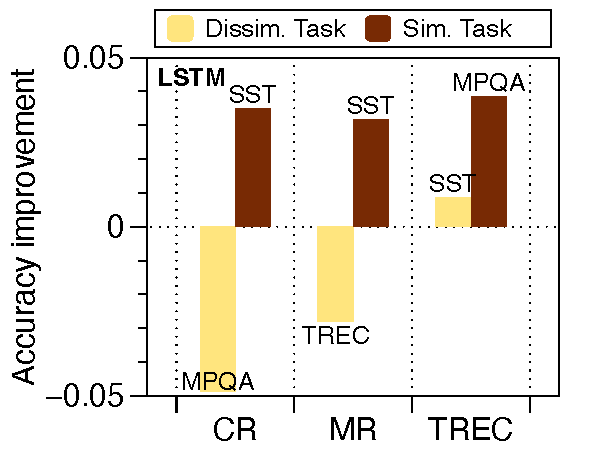
\includegraphics[width=0.975\textwidth]{figures/task_sim_norm_lstm.pdf}
%		\caption{Task similarity}
%		\label{fig_ab_sim}
%	\end{subfigure}%
%	\caption{Validating the three results of Section \ref{sec_insight} on sentiment analysis tasks. (a) Adding a semantically similar source task in MTL performs better than adding a dissimilar task.
%	(b) As source/target sample ratio increases, we observe a transition from positive to negative transfer.
%	(c)
%	Note: (S) denotes the source task and (T) denotes the target task.}


%\begin{minipage}[t]{.58\textwidth}
%	\vspace{-0.1in}
%	\centering
%  \begin{tabular}{c c c c c}
%	\toprule
%		\multirow{2}{*}{{\bf Threshold}}  & \multicolumn{2}{c}{{\bf Sentiment
%		analysis}} & \multicolumn{2}{c}{{\bf ChestX-ray14}} \\
%		& Precision &  Recall & Precision &  Recall \\
%		\cmidrule(lr){1-1} \cmidrule(lr){2-3} \cmidrule(lr){4-5}
%		0.0 & 0.596 & 1.000 & 0.593 & 1.000 \\
%		0.1 & \textbf{0.756} & \textbf{0.388} & \textbf{0.738} & \textbf{0.462} \\
%		0.2 & 0.919 & 0.065 & 0.875 & 0.044 \\
		% 0.3 & 1.000 & 0.004 &     - &     - \\
%	\bottomrule
%	\end{tabular}
%	\vspace{0.1in}
%	\captionof{table}{Single-task learning results can help predict postive or negative transfer in multi-task learning.}
%	\label{tab:mtl_better_than_stl}
%\end{minipage}%
%\quad



%\begin{figure}[!t]
%	\centering
%	\begin{subfigure}[b]{0.5\textwidth}
%		\centering
%		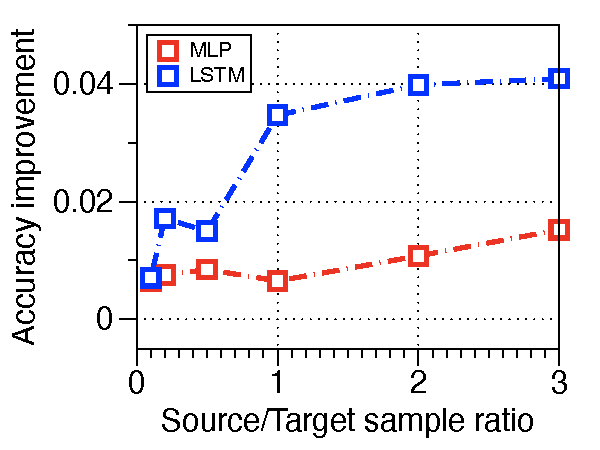
\includegraphics[width=0.5\textwidth]{figures/ratio_alignment_norm_diff_all.pdf}
%		\caption{Averaged over all 16 task pairs}
%		\label{fig_ab_cov}
%	\end{subfigure}\hfill
%	\begin{subfigure}[b]{0.5\textwidth}
%		\centering
%		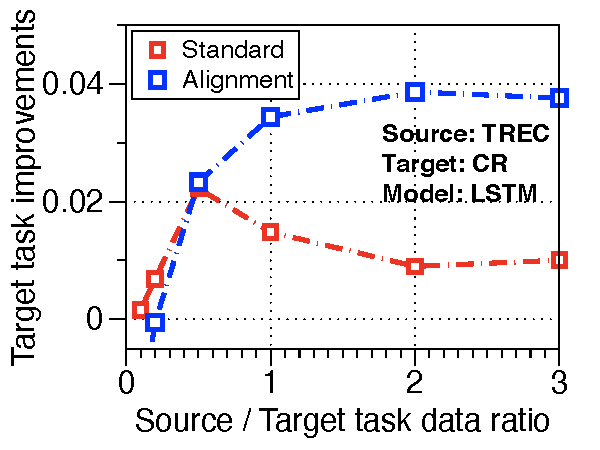
\includegraphics[width=0.5\textwidth]{figures/ratio_alignment_norm_trec_cr_lstm.pdf}
%		\caption{An example task pair}
%		\label{fig_cov_a}
%	\end{subfigure}
%	\caption{ (TREC and CR)}
%\end{figure}

%\textbf{Further results of the covariance alignment procedure.}
%Our results in Figure \ref{fig_ab_cov} are averaged over all the task pairs.
%In Figure \ref{fig_covariate_app}, we show two task pairs as examples.
%In Figure \ref{fig_cov_a}, we observe that for the particular task pair, covariance alignment provides more significant gains when the sample ratio is large.
%In Figure \ref{fig_cov_b}, we observe that covariance alignment does not always improve over the baseline multi-task learning model.
%One explanation is that MR and SST are similar tasks, hence adding the alignment module is unnecessary.
%An interesting question is to understand when adding the alignment module benefits the multi-task learning model.
%We leave this question for future work.
%Note: For text classification tasks, the source task training data size ranges from 500 to 1,500 and target task training data size is 1000; For ChestX-ray14,

%\begin{figure}[!h]
%	\centering
%	\begin{subfigure}[b]{0.48\textwidth}
%		\centering
%		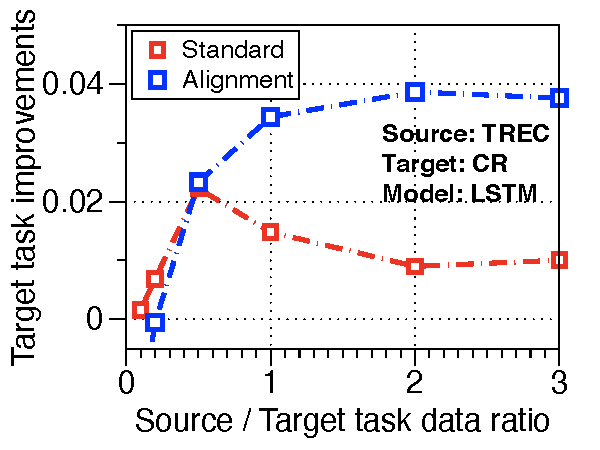
\includegraphics[width=0.7\textwidth]{figures/ratio_alignment_norm_trec_cr_lstm.pdf}
%		\caption{Task pair TREC and CR}
%		\label{fig_cov_a}
%	\end{subfigure}\hfill
%		\begin{subfigure}[b]{0.48\textwidth}
%		\centering
%		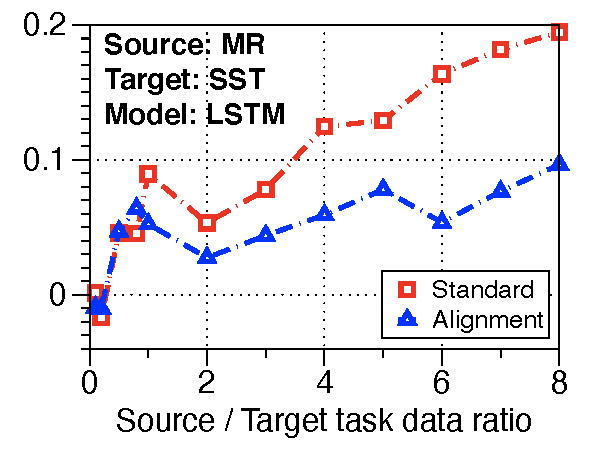
\includegraphics[width=0.7\textwidth]{figures/ratio_alignment_mr_sst_lstm.pdf}
%		\caption{Task pair MR and SST}
%			\label{fig_cov_b}
%	\end{subfigure}
%	\caption{(a) For the task pair TREC and CR, adding the covariance alignment procedure provides more improvement when the source/target sample ratio is large.
%	(b) For the task pair MR and SST, adding the covariance alignment procedure hurts performance.
%	One explanation is that MR and SST are similar tasks, hence adding the alignment module is unnecessary.}
%	\label{fig_covariate_app}
%\end{figure}


\begin{figure}%[!t]
	\begin{subfigure}[t]{0.5\textwidth}
		\centering
		\vspace{0pt}
		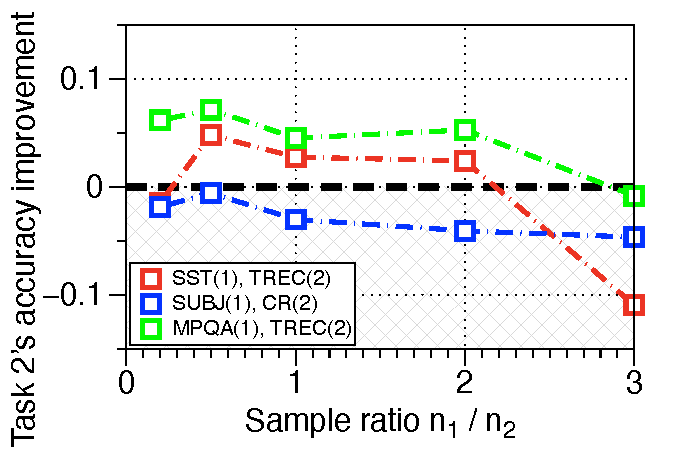
\includegraphics[width=0.8\textwidth]{figures/fig3a.pdf}
		\caption{HPS vs. STL}
		\label{fig_ab_data}
	\end{subfigure}\hfill
	\begin{subfigure}[t]{0.5\textwidth}
		\centering
		\vspace{0pt}
		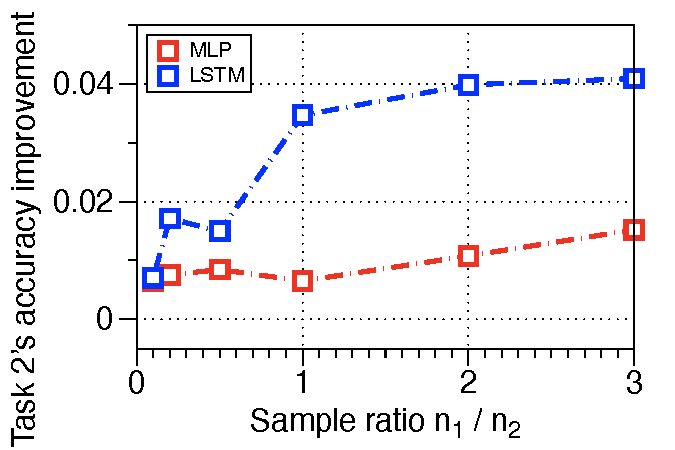
\includegraphics[width=0.8\textwidth]{figures/fig3b.pdf}
		\caption{HPS vs. covariance alignment}
		\label{fig_ab_cov}
	\end{subfigure}
	\caption{Comparing hard parameter sharing (HPS) to single-task learning (STL) and a covariance alignment approach proposed by \cite{WZR20}:
	In Figure \ref{fig_ab_data}, we observe that for multiple task pairs, increasing task one's sample size improves task two's prediction accuracy initially, but hurts eventually -- a phenomenon similar  to Figure \ref{fig_size}.
	In Figure \ref{fig_ab_cov}, we observe that as task one's sample size increases, covariance alignment improves more over HPS.}
	\label{fig_text}
%	\begin{minipage}[t]{0.4\textwidth}
%		\centering
%		\vspace{0pt}
%		\begin{tabular}{c c c}
%		\toprule
		% \multirow{2}{*}{{\bf Models}} & \multicolumn{2}{c}{\begin{minipage}{1.2in}\begin{center}
		% Sentiment\\ analysis\end{center}\end{minipage}} \\
%		\multirow{2}{*}{{\bf Models}} & \multicolumn{2}{c}{\bf Sentiment analysis} \\
		% \cmidrule(lr){2-3}
%		& all tasks & w/o TREC \\
%		\midrule
%		{\bf MLP}  & 31\% & 29\% \\
%		{\bf LSTM} & 35\% & 34\% \\
%		{\bf CNN}  & 30\% & 28\% \\
%		\bottomrule
%		\end{tabular}
%		\captionof{table}{Finding the best sample ratio via a progressive training schedule.}
%		\label{tab:taskonomy}
%	\end{minipage}
\end{figure}

%\begin{algorithm}[!t]
%	\caption{A progressive training schedule given two tasks}
%	\label{alg_inc_train}
%	\begin{algorithmic}[1]
%		\Input Two tasks $(X^{(1)}, Y^{(1)})$ and $(X^{(2)}, Y^{(2)})$.
%		\Param A shared module $B$, output layers $A_1, A_2$ as in the hard parameter sharing architecture.
%		\Req \# batches $S$, epochs $T$, task $2$'s validation accuracy $\hat{g}(B; W_2)$, a threshold $\tau\in(0,1)$.
%		\Output The trained modules $B, A_2$ optimized for task $2$.
%		\State Divide $(X^{(1)}, Y^{(1)})$ randomly into $S$ batches: $(x^{(1)}, y^{(1)}), \dots, (x^{(S)}, y^{(S)})$.
%		\For{$i = 1,\dots, S$}
%			\For{$j = 1,\dots, T$}
%				\State Update $B, A_1, A_2$ using the training data $\set{x^{(k)}, x^{(k)}}_{k=1}^i$ and  $(X^{(2)}, Y^{(2)})$.
%			\EndFor
%			\State Let $a_i = \hat{g}(B; A_2)$ be the validation accuracy.
%			\If{$a_i < a_{i-1}$ or $a_i > \tau$}
%				\State \textbf{break}
%			\EndIf
%		\EndFor
%	\end{algorithmic}
%\end{algorithm}